\chapter{Psychohry}

Hrou je myšlen souvislý sled druhotných doplňkových transakcí, které vedou k definovanému předem známému výsledku. 
Od ostatních typů transakcí (zábavy, rituály) se liší především dvěma hlavními rysy - vedlejšími vlastnostmi a předem daným výsledkem. 
Hry oproti ostatním transakcím často obsahují konfliktní prvky.
Protože každodenní život nenabízí velké množství příležitostí pro složené intimní vztahy, jsou hry velmi rozšířenou skupinou interakcí ve společnosti.
Hlavním účelem her je jejich výsledek, ačkoliv vedlejším a neméně důležitým produktem her je pocit uspokojení pro alespoň jednoho hráče.
Podstatou her jsou  vedlejší vlastnosti (transakce), které vedou k zisku a umožňují hráčům udržet si duševní rovnováhu a jednotlivé kroky hry jsou "pouze" kroky k dosažení cíle \cite{jak_si_lide_hraji}.\\

Každá hra má čtyři fáze. Začíná fintou, ve které hráč chytí druhého na nějakou slabost. 
Následuje odhalení karet, o co hráči jde. 
Na toto navazuje navození zmatku, kterývede k výhře hráče. 
Výhra může mít různou podobu - pocity nadřazenosti, převahy, pýchy, ale i zmaru a beznaděje \cite{translacni_analyza_prirucka}.\\

Na klasifikaci her lze pohlížet z různých hledisek \cite{jak_si_lide_hraji}:
    \begin{itemize}
        \item Počet hráčů: dvoučlenná (Frigidní žena), tříčlenná hra (Ať si to spolu rozdají), pětičlenná hra (Alkoholik) a vícečlenná hra (A nemohl byste -- Ano, ale).
        \item Užívané rekvizity: slova (Psychiatrie), peníze (Dlužník), části těla (Poliklinika).
        \item Klinické typy: hysterický (Hra s ohněm), obsedantně kompulzivní (Kazisvět), paranoický (Že já mám věčně takovou smůlu!), depresivní (Už jsem v tom zas).
        \item Zóna: orální (Alkoholik), anální (Kazisvět), falická (Ať si to spolu rozdají).
        \item Psychodynamika: antifobická (Kdyby nebylo tebe), projektivní (Rodičovské sdružení), introspektivní (Psychiatrie).
        \item Instinkty: masochistický (Kdyby nebylo tebe), sadistický (Kazisvět), fetišistický (Frigidní žena).
        \item Pružnost: jak pružně lze volit různé rekvizity, některé hry lze hrát jen s danou sadou rekvizit, u některých lze být kreativnější.
        \item Vytrvalost: jak dokážou lidé zanechat svých her, zda se jich pevně drží nebo jich mohou lehce zanechat.
        \item Intenzita - mírné a tvrdé: klasifikace dle útočnosti hráčů během hry
        \item Hra prvního stupně: je v okolí hráče společensky přijatelná.
        \item Hra druhého stupně: nepůsobí v okolí trvalou, nenapravitelnou škodu, hráči ji však raději hrají v ústraní, mimo veřejnost.
        \item Hra třetího stupně: se hraje na výdrž a končí buď v nemocnici, v soudní síni nebo v márnici.
    \end{itemize}{}
    
Existují další klasifikace her a sám Berne používal sociologickou klasifikaci, takto klasifikoval přes 35 her:
    \begin{itemize}
        \item Životní hry - alkoholik, dlužník, kopejte do mě, POTYDA - počkej, ty darebáku - já ti úkážu, VIČEDO - Vidíš, k čemu jste mě dohnali!
        \item Manželské hry - kout, soud, fritidní žena, otrokyně, drahoušek, KDYMET - Kdyby nebylo tebe, vidíš, jak se obětuji
        \item Společenské hry - vrták, kazisvět, TOJEHR - To je hrozné, viďte?, ANEBY - A nemohl byste -- Ano, ale
        \item Sexuální hry - perverze, hra s ohněm, hra s punčochou, kravál, ASPRO - Ať si to spolu rozdají
        \item Hry podsvětí - jak vzít roha, ZAP - zloději a policajti, VEHUL - Teď ho vezmeme na hůl
        \item Hry v poradnách - skleník, sociální případ, naivka, psychiatrie, budižkničemu, protéza, MYTODO - Myslím to s vámi dobře
        \item Neškodné hry - odborník na dovolené, kavalír, dobrodinec, všeuměl, ještě budou rádi, že mne poznali
    \end{itemize}{}

Vypisovat všechny hry a jejich zákonitosti by bylo zbytečné. Jejich popis je v Berneho knize Jak si lidé hrají \cite{jak_si_lide_hraji} a zde přikládám přehlednou tabulku ze závěrečné práce Antonína Svabady \cite{svabada_tabulka}.\\

    \begin{figure}
        \centering
        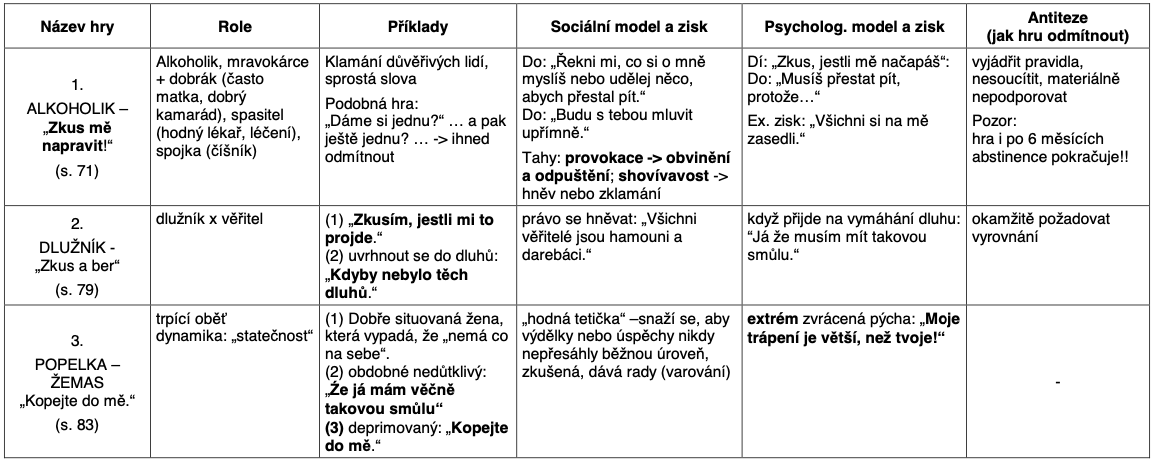
\includegraphics[width=\textwidth]{pictures/1.png}
        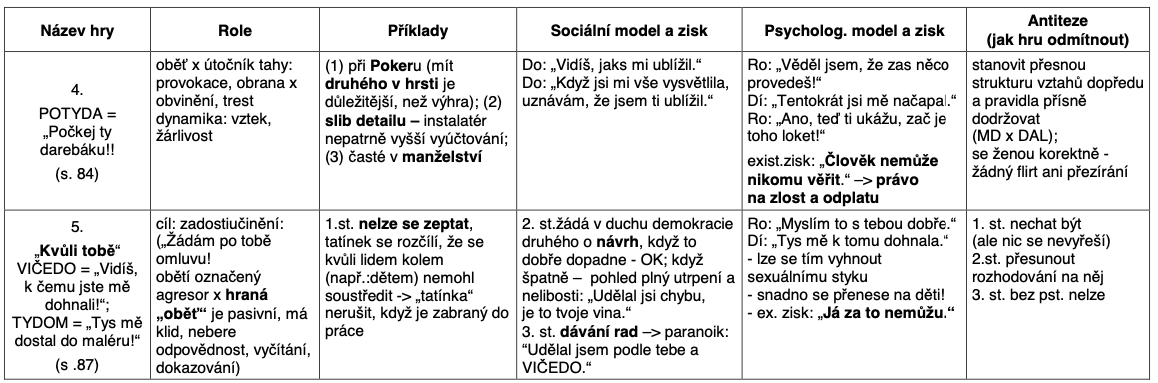
\includegraphics[width=\textwidth]{pictures/2.png}
        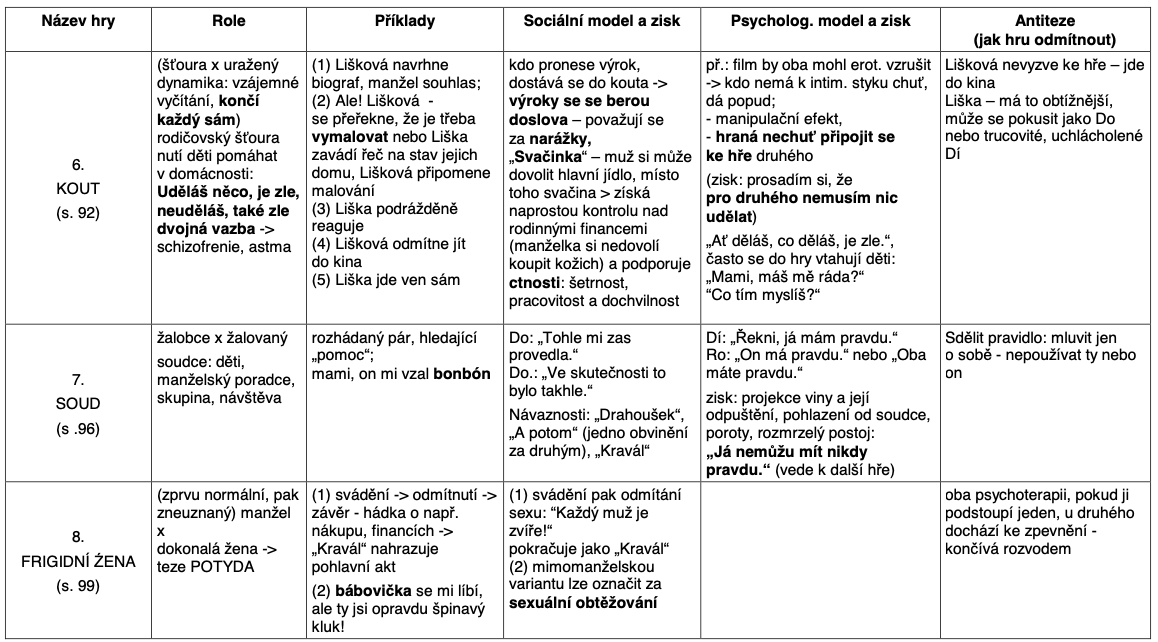
\includegraphics[width=\textwidth]{pictures/3.png}
    \end{figure}{}

    \begin{figure}
        \centering
        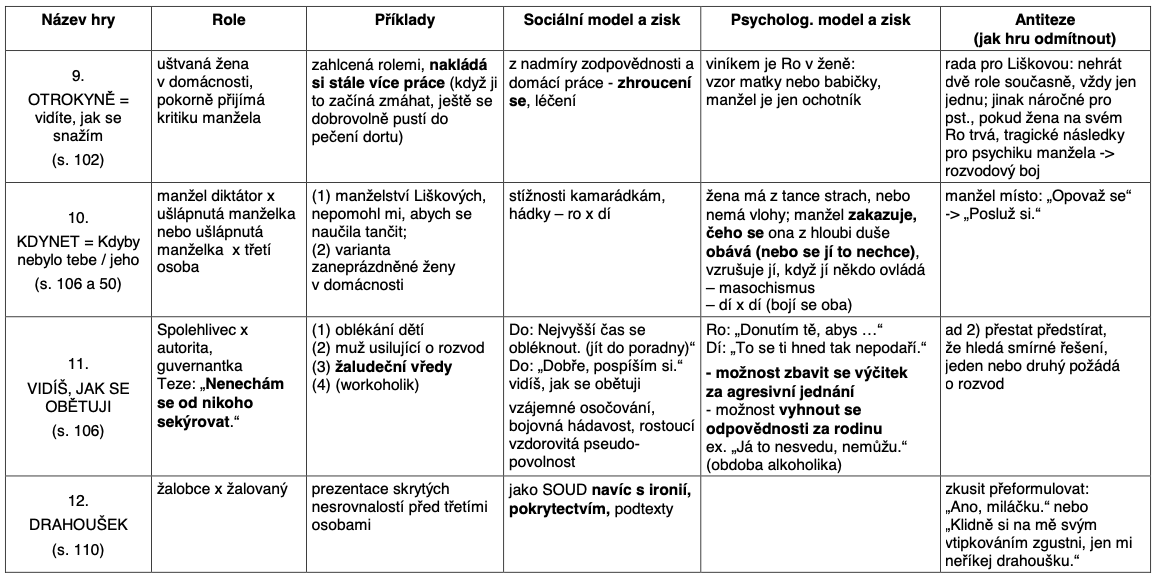
\includegraphics[width=\textwidth]{pictures/4.png}
        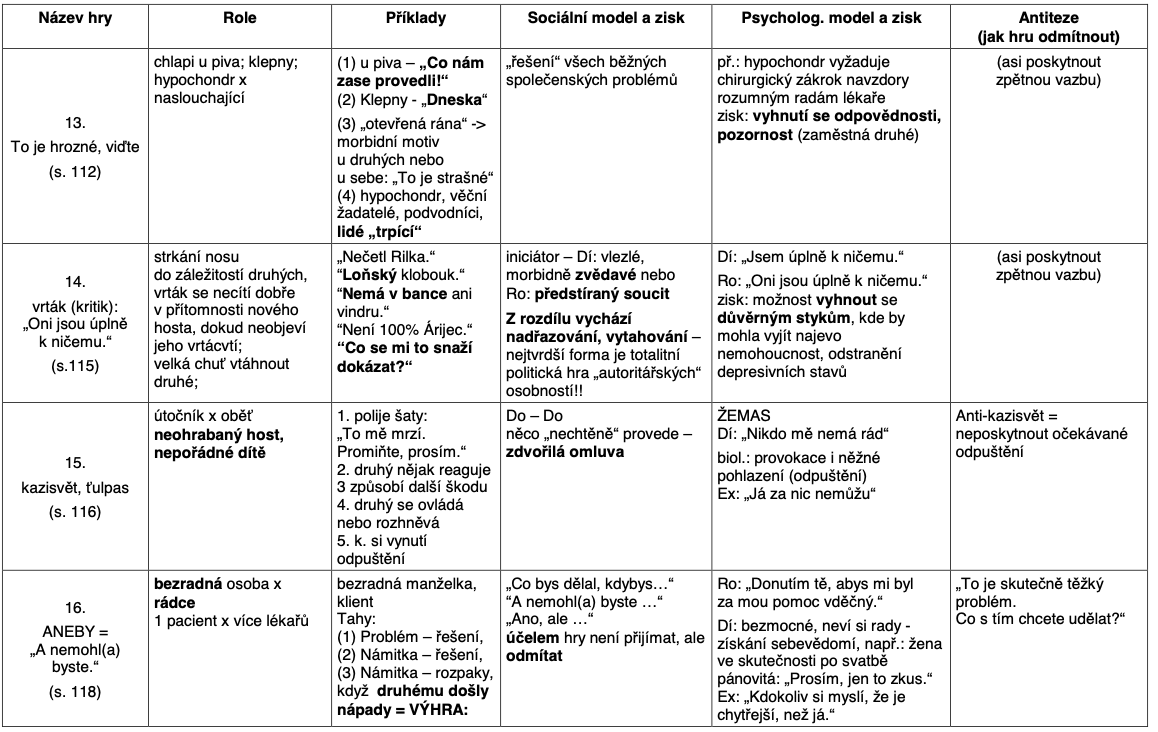
\includegraphics[width=\textwidth]{pictures/5.png}
    \end{figure}{}
    
    \begin{figure}
        \centering
        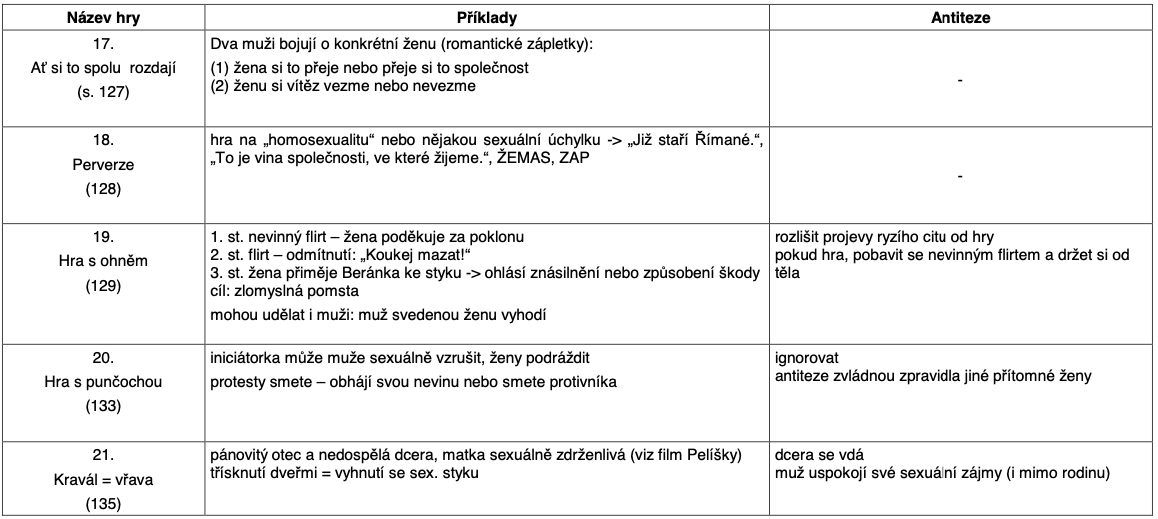
\includegraphics[width=\textwidth]{pictures/6.png}
        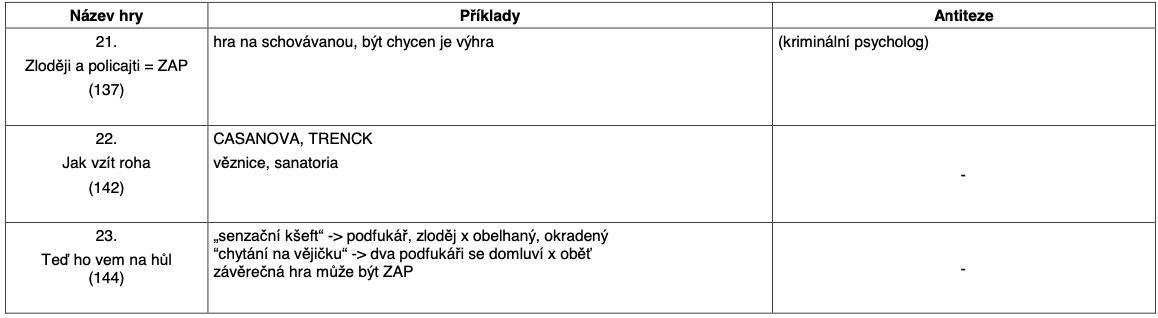
\includegraphics[width=\textwidth]{pictures/7.png}
        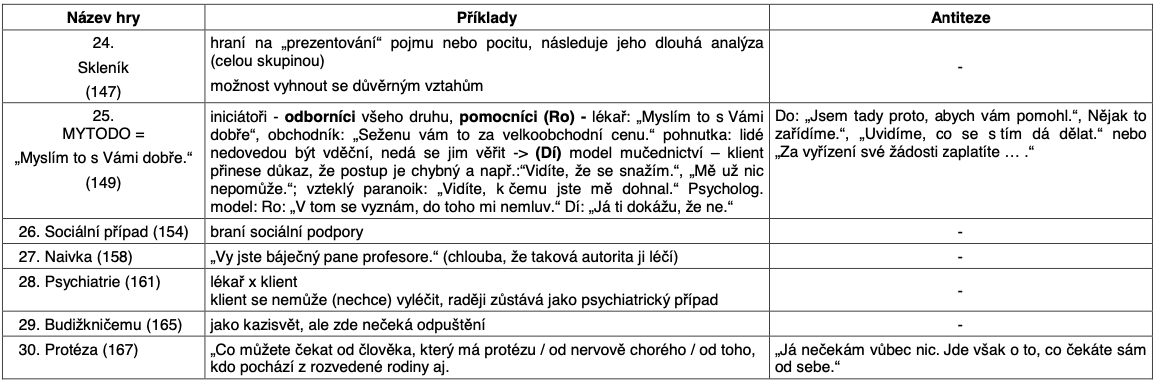
\includegraphics[width=\textwidth]{pictures/8.png}
        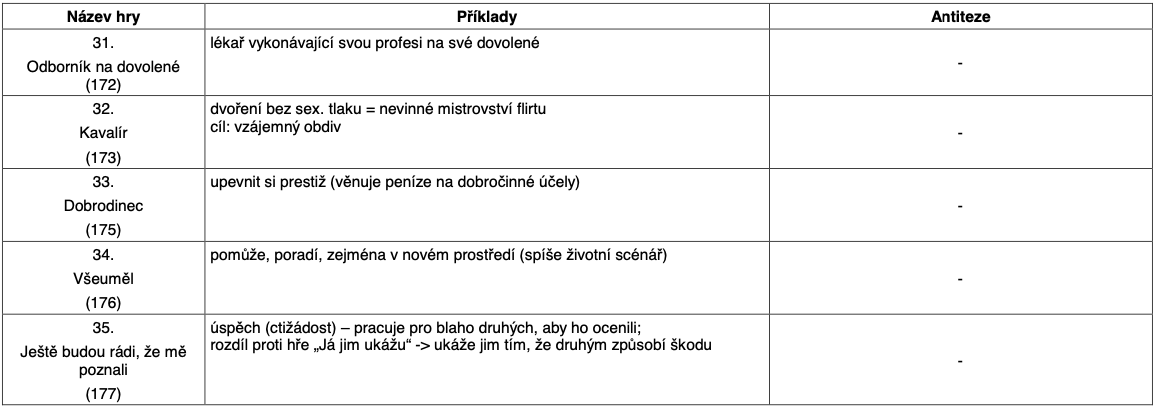
\includegraphics[width=\textwidth]{pictures/9.png}
    \end{figure}{}
\chapter{Závěr}

V práci pana Svabady stejně jako na konkrétních příkladech pana Berna je názorně ukázáno, jak může být hraní her destruktivní a zákeřné. Transakční analýza umožňuje podrobně analyzovat chování jedince. Je jistě vhodné se nad vlastní analýzou osobnosti zamyslet. Jaký ego-stav je pro nás tím směřujícím, jestli to je opravdu Dospělý nebo naopak Rodič či Dítě. \\

Je až překvapivé, kolik a jakých her jsou  součástí běžné společnosti. Berne a jeho příznivci rozvinuli transakční analýzu do podoby vhodné terapeutické metody léčby psychologických poruch nejen pro individuální léčbu, ale také pro skupinovou terapii.\\

Během studia literatury k vypracování seminární práce, jsem byla překvapena použitelností a praktičností transakční analýzy a z pohledu laika bych knihy pana Berna doporučila čtenáři nejen jako zdroj odborných znalostí, ale také jako poměrně čtivou, realistickou a humornou literaturu.


